\documentclass[conference,compsoc,final,a4paper]{IEEEtran}
\usepackage[utf8]{inputenx}

%% Bitte legen Sie hier den Titel und den Autor der Arbeit fest
\newcommand{\autorA}[0]{Büchner, Jannis}
\newcommand{\autorB}[0]{Büchner, Niklas}
\newcommand{\autorC}[0]{Vierling, Jörg}
\newcommand{\dokumententitel}[0]{Tik-Tak-Toe Roboter}

% Hie muss normalerweise nichts angepasst werden
\usepackage[pdftex]{graphicx}
\graphicspath{{img/}}
\DeclareGraphicsExtensions{.pdf,.jpeg,.jpg,.png}
\usepackage[cmex10]{amsmath}
\usepackage{algorithmic}
\usepackage{array}
\usepackage{dblfloatfix}
\usepackage{url}
\usepackage[autostyle=true,german=quotes]{csquotes}
\usepackage[backend=biber,
            sorting=none,   % Keine Sortierung
            doi=true,       % DOI anzeigen
            isbn=false,     % ISBN nicht anzeigen
            url=true,       % URLs anzeigen
            maxnames=6,     % Ab 6 Autoren et al. verwenden
            minnames=1,     % und nur den ersten Autor angeben
            style=ieee,]{biblatex}
\usepackage{booktabs}
\usepackage{xcolor}
\usepackage{listings}             % Source Code listings
\usepackage[printonlyused]{acronym}
\usepackage{fancyvrb}
\usepackage{tocloft} % Schönere Inhaltsverzeichnisse
\usepackage{amsmath}
\usepackage{siunitx}
\usepackage{booktabs}


% Farben definieren
\definecolor{linkblue}{RGB}{0, 0, 100}
\definecolor{linkblack}{RGB}{0, 0, 0}
\definecolor{darkgreen}{RGB}{14, 144, 102}
\definecolor{darkblue}{RGB}{0,0,168}
\definecolor{darkred}{RGB}{128,0,0}
\definecolor{comment}{RGB}{63, 127, 95}
\definecolor{javadoccomment}{RGB}{63, 95, 191}
\definecolor{keyword}{RGB}{108, 0, 67}
\definecolor{type}{RGB}{0, 0, 0}
\definecolor{method}{RGB}{0, 0, 0}
\definecolor{variable}{RGB}{0, 0, 0}
\definecolor{literal}{RGB}{31,0, 255}
\definecolor{operator}{RGB}{0, 0, 0}

\usepackage[ngerman]{betababel}

\DefineBibliographyStrings{ngerman}{
    andothers = {{et al\adddot}},  % Immer et al. sagen, auch bei Deutsch als Sprache
}
\usepackage[
      unicode=true,
      hypertexnames=false,
      colorlinks=true,
      colorlinks=false,
      linkcolor=darkblue,
      citecolor=darkblue,
      urlcolor=darkblue,
      pdftex
   ]{hyperref}
%	 \PrerenderUnicode{ü}


% Einstellungen für Quelltexte
\lstset{
    xleftmargin=0.1cm,
    basicstyle=\scriptsize\ttfamily,
    keywordstyle=\color{keyword},
    identifierstyle=\color{variable},
    commentstyle=\color{comment},
    stringstyle=\color{literal},
    tabsize=2,
    lineskip={2pt},
    columns=flexible,
    inputencoding=utf8,
    captionpos=b,
    breakautoindent=true,
    breakindent=2em,
    breaklines=true,
    prebreak=,
    postbreak=,
    numbers=none,
    numberstyle=\tiny,
    showspaces=false,      % Keine Leerzeichensymbole
    showtabs=false,        % Keine Tabsymbole
    showstringspaces=false,% Leerzeichen in Strings
    morecomment=[s][\color{javadoccomment}]{/**}{*/},
    literate={Ö}{{\"O}}1 {Ä}{{\"A}}1 {Ü}{{\"U}}1 {ß}{{\ss}}2 {ü}{{\"u}}1 {ä}{{\"a}}1 {ö}{{\"o}}1
}

\hypersetup{
    pdftitle={\dokumententitel},
    pdfauthor={\autoren},
    pdfdisplaydoctitle=true,
    hidelinks
}

% Makros für typographisch korrekte Abkürzungen
\newcommand{\zb}[0]{z.\,B.\ }
\newcommand{\dahe}[0]{d.\,h.\ }
\newcommand{\ua}[0]{u.\,a.\ }

% Wo liegt Sourcecode?
\newcommand{\srcloc}{src/}

% Literatur einbinden
\addbibresource{literatur.bib}
 % Weitere Einstellungen aus einer anderen Datei lesen

\begin{document}

% Titel des Dokuments
\title{\dokumententitel}

% Namen der Autoren
\author{
  \IEEEauthorblockN{
    \autorA\\
    \autorB\\
    \autorC
  }
  \IEEEauthorblockA{
    Hochschule Mannheim\\
    Fakultät für Informatik\\
    Paul-Wittsack-Str. 10,
    68163 Mannheim
    }
}

% Titel erzeugen
\maketitle
\thispagestyle{plain}
\pagestyle{plain}

% Eigentliches Dokument beginnt hier
% ----------------------------------------------------------------------------------------------------------

% Kurze Zusammenfassung des Dokuments
\begin{abstract}
An dieser Stelle steht eine kurze Zusammenfassung des Inhaltes des Dokuments. Der Abstrakt ist vollkommen eigenständig und hat weder Querverweise zu anderen Teilen dieser Arbeit noch Referenzen zu Quellen.

Schreiben Sie die Zusammenfassung im sogenannten faktenzentrierten Stil, d.\,h. beschreiben Sie nicht das Dokument, sondern die Fakten und Informationen, die das Dokument liefert. Zum Beispiel schreiben Sie \textit{nicht} \enquote{Dieses Dokument stellt die besondere Bedeutung des Flux-Kompensators für Zeitreisen im Film \enquote{Zurück in die Zukunft} dar.}, sondern schreiben Sie \enquote{Ohne den Flux-Kompensator wären die Zeitreisen im Film \enquote{Zurück in die Zukunft} nicht möglich.}

Den Abstract schreibt man als letztes.
\end{abstract}

% Inhaltsverzeichnis erzeugen
{\small\tableofcontents}

\section{Projektziel}

\begin{itemize}
  \item Tik-Tak-Toe Roboter
  \item Warum Tik-Tak-Toe
  \item Roboter, der sich auf 3 Achsen bewegen kann (a.k.a. Plotter)
\end{itemize}

Ziel dieses Projektes war es einen kleinen Roboter zu entwickeln, der Tik-Tak-Toe
auf einem Blatt Papier gegen den Nutzer spielen kann. Hierbei wurde Tik-Tak-Toe
gewählt, da es ein simples aber sehr bekanntes Spiel ist.

Das Team hat sich gegen die Nutzung eines schon existierenden Roboters oder Roboter-Kit
entschieden, um mit allen Bereichen der Robotik in Kontakt zu kommen. Ziel war es hier
eine Fachschafts übergreifende Kooperation zu nutzen, um einen optimalen Wissenstransfer
zu erreichen.

Um das Spiel Tik-Tak-Toe spielen zu können soll der Roboter in der Lage sein das Spielfeld
sowie die Züge aller Spieler zu zeichen. Daraus ergab sich die grundsätzlichen Anforderung
an die Hardware, dass sie eine Bewegung in alle drei Raumrichtungen unabhängig voneinander
ermöglichen muss. Zudem sollte diese robust gestaltet und einfach zu realisieren sein.
Deswegen wurde entschieden einen Plotter zu bauen anstelle eines komplizierteren
Roboterarms. Dies hatte vor allem den Vorteil, dass die Bewegungen einfach zu realisieren
sind, ohne komplizierte Koordinatentransformationen durchführen zu müssen.


\section{Mechanik}

\begin{itemize}
  \item Roboter, der sich auf 3 Achsen bewegen kann
  \item ESP32 vs andere Chips
  \item Warum Fischertechnik
  \item Schaltplan
  \item Zu lösende Probleme:
    \begin{itemize}
      \item Koordination Bewegungen
      \item Drehmoment, Geschwindigkeit
    \end{itemize}
\end{itemize}

Da zu Beginn des Projekts kein Roboter vorhanden war, musste nicht nur der Code geschrieben, sondern auch die Hardware konstruiert werden. Die grundsätzlichen Anforderungen an die Hardware waren, dass sie eine Bewegung in alle drei Raumrichtungen unabhängig voneinander ermöglichen muss, robust gestaltet und einfach zu realisieren sein sollte. Deswegen wurde entschieden einen Plotter zu bauen anstelle eines komplizierteren Roboterarms. Dies hatte vor allem den Vorteil, dass die Bewegungen einfach zu realisieren sind, ohne komplizierte Koordinatentransformationen durchführen zu müssen.

Um den Plotter zu bauen wurde Fischertechnik eingesetzt. Zum einen waren davon schon Teile vorhanden, zum anderen erfüllen diese Materialien die Anforderungen an Robustheit ausreichend. Des Weiteren lass sich lineare Bewegungen mithilfe von Spindelgetrieben oder Kegelzahnräder einfach realisieren lassen. 
Die Spindelgetriebe haben den Vorteil, dass sie aus einzelnen Schneckenteilen bestehen, die nacheinander auf eine Achse geschoben werden und dadurch in verschiedenen Längen konstruiert werden können. Damit die Schneckenteile nicht verrutschen befinden sich an den Enden klemmbare Schnecken, die mithilfe von Spannzangen fixiert werden. Letztlich befindet sich an jeder Achse noch ein Zahnrad, das zum Antrieb des Spindelgetriebe genutzt wird.

Die Bewegungen in x, y und z-Richtung werden separat voneinander gesteuert. Im Prinzip ist der Plotter somit aus drei Schichten aufgebaut. Die unterste Schicht, der Grundrahmen, ist für die Bewegung in x-Richtung, also vor und zurück, zuständig. Darauf sitzen zwei y-Schlitten, die die mittlere Schicht darstellen. Diese sorgt für die Bewegung nach links und rechts, in y-Richtung. Darauf sitzt der Stiftehalter, der in z-Richtung nach oben und unten bewegt werden kann.

Der Grundrahmen besteht aus jeweils einer Achse und einem Spindelgetriebe, die sich links und rechts am Plotter befinden und an den Enden auf zwei Basisplatten befestigt sind. Auf jedem Paar aus Achse und Spindelgetriebe befindet sich ein y-Schlitten, welcher durch die Drehbewegung des Spindelgetriebes nach vorne und hinten bewegt wird. Die Aufgabe der Achsen ist die Lasten und Momente aufzunehmen. Ein Aufbau aus nur einem Spindelgetriebe und zwei Achsen hätte zur Folge, dass entweder das zu kompensierende Drehmoment sehr groß gewesen wäre, wenn beide Achsen auf derselben Seite des Plotters angebracht worden wären oder die zwei Schlitten, sich nicht gleichmäßig bewegt hätten, sondern verzogen hätten, wären die Achsen auf unterschiedlichen Seiten des Plotters angebracht worden. Eine zweite Achse musste aber unbedingt eingebaut werden, weil sonst das Getriebe das Drehmoment kompensieren müsste, wofür es aber nicht geeignet ist.
Damit sich die Spindelgetriebe gleich schnell und gleichzeitig drehen, sind diese mithilfe von einer Kette (bestehend aus einzelnen Rastkettengliedern) verbunden. Dadurch wird eine gleichmäßige Bewegung gewährleistet und die Schlitten, die obendrauf sitzen, verziehen sich nicht. Die Bewegung in x-Richtung wird durch einen XM-Motor von Fischertechnik ausgeführt, welcher auf einer Basisplatte sitzt und eine der Getriebe mithilfe von Zahnrädern antreibt. Das Zahnrad an der Antriebswelle wurde so klein wie möglich gewählt, im Vergleich zum Zahnrad an der Getriebewelle. Der Grund dafür ist, dass dadurch die Drehzahl reduziert wird, und die Schlitten sich nicht zu schnell bewegen und dass das Drehmoment nochmal zusätzlich erhöht wird, um mechanische Ungenauigkeiten, die zu einem größeren Widerstand führen, zu kompensieren. Ein Problem mit der Anordnung des Motors und des kleinen Zahnrades ist, dass die Antriebswelle nicht fixiert werden kann und sich erstmal schräg stellt, bevor das große Zahnrad anfängt sich zu drehen. Jegliche Idee die Welle zu fixieren hätte dazu geführt, dass die Konstruktion an der Kette reibt. Um dieses Problem zu lösen hätte es größere Umbauten am gesamten Plotter benötigt, die aufgrund des späten Zeitpunktes, zu dem der Motor angekommen ist, nicht mehr möglich waren. 

Die zwei y-Schlitten sind ebenfalls mit zwei Achsen und einem Spindelgetriebe verbunden. Auch hier nehmen die Achsen das Gewicht sowie das resultierende Drehmoment des Stiftehalter auf. Im Gegensatz zum Aufbau in x-Richtung befinden sind diese übereinander angeordnet, damit der Aufbau nicht zu sehr nach vorne ragt, sondern stattdessen in die Höhe. Der Nachteil dabei ist aber, dass sich der Stift nicht zwischen den Achsen befindet, was zu einem exzentrischen Kraftfluss führt und somit ein größeres Drehmoment nach sich zieht. 
Der Motor (Motor XS von Fischertechnik), der die y-Bewegung ausführt, ist etwas leistungsschwacher als der für die x-Bewegung. Dies hat den Vorteil, dass er sehr viel kleiner und leichter ist. Dadurch kann er direkt auf einem der zwei y-Schlitten angebracht werden, ohne ein Ungleichgewicht zu erzeugen. Auch hier wird die Kraftübertragung zwischen der Antriebswelle des Motors und der Abtriebwelle des Spindelgetriebes mithilfe von Zahnrädern ermöglicht. 

Auf der y-Achse befindet sich ein weiterer Schlitten, der im Großen und Ganzen aus zwei Teilen besteht. 
Der eine Teil ist für das Anheben und Absetzen des Stiftes zuständig. Dieser besteht aus einer Rastachse mit Schnecke, die über Kegelzahnräder bewegt wird. Auf der Schnecke befindet sich eine Schneckenmutter, deren Drehbewegung verhindert wird, indem sie an einem Klotz festgemacht ist, durch den eine parallele Achse geht. Dadurch werden die Mutter und der Klotz gezwungen sich nach oben und unten zu bewegen. An dem Klotz befindet sich der Stiftehalter. Das Ziel bei der Konstruktion des Stiftehalter war, ein einfacher, effizienter und effektiver Aufbau, mit dem der Stift sowohl angehoben als auch mit Druck abgesetzt werden kann. Des Weiteren sollte es möglich sein, viele verschiedenen Arten von Stifte zum Spielen verwenden zu können. Die beste Lösung für dieses Problem war den Stift mithilfe von Tesa-Film an zwei aneinander befestigte Bausteine zu kleben. 
Das Kegelzahnrad an der Schnecke wird durch einen XS Motor von Fischertechnik bewegt. Dieser befindet sich ebenfalls auf dem Schlitten.
Der zweite Teil des Schlittens besteht aus einer Konstruktion, die verhindern soll, dass der Stift sich zu sehr verbiegt. Die L-förmige Konstruktion liegt von allen Seiten press am Stift und ist direkt mit dem Schlitten und den Achsen verbunden. Sie bewegt sich nicht mit dem Stift nach oben und unten. Dass der Stift sich leicht verbiegt, lässt sich nicht verhindern aber dadurch stark einschränken.

\section{Elektrik}
Aufgrund der vorangegangenen Entscheidung, den ESP32-WROVER zu verwenden, basiert der Aufbau der elektrischen Schaltung auf dem Stecksystem des ESP32-WROVER-Boards.

\subsection{Aufbau der Versuchsumgebung}
\begin{figure}[h]
\centering
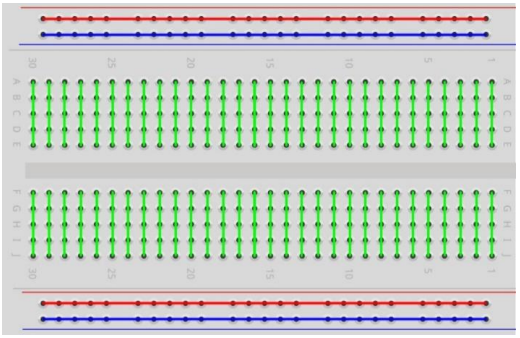
\includegraphics[width=8.5cm]{../images/board.png}
\caption{Aufbau Entwicklungs-Board}
\label{Elektrik:DevBoard}
\end{figure}
\begin{figure}[h]
\centering
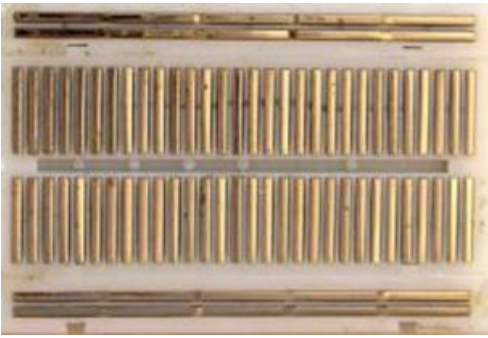
\includegraphics[width=8.5cm]{../images/board2.png}
\caption{Schaltung Entwicklungs-Board}
\label{Elektrik:DevBoardInternal}
\end{figure}

In den Abbildung 1 und 2 sind die einzelnen Leiterbahnen zu sehen, auf welchen die einzelnen Bauteile platziert werden können (grüne Linien). 
Dieser Aufbau ermöglicht bis zu 5 direkte Verbindungen innerhalb einer Leiterbahn und insgesamt 60 elektrisch voneinander getrennte Leitungen.

Die äußeren Leiterbahnen sind für die Spannungsversorgung vorgesehen und erstrecken sich über das gesamte Board. Diese Leiterbahnen werden mit 5 V bzw. 3,3 V betrieben.
Die Verbindungen zwischen dem Micro-Controller und dem Entwicklungsboard wird mithilfe eines Extension Boards hergestellt. Das Extension Board ist so konzipiert, 
dass die einzelnen Pins des Micro-Controllers mit bestimmten Leiterbahnen auf dem ESP32-WROVER-Boards verbunden werden.

Zu beachten ist hierbei das Insgesamt 40 Leiterbahnen somit nicht frei benutzt werden können, da diese eine direkte Verbindung mit Micro-Controller darstellen.
\begin{figure}[h]
\centering
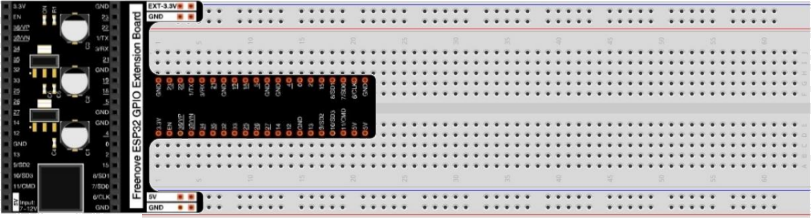
\includegraphics[width=8.5cm]{../images/ext_board.png}
\caption{Schaltung Entwicklungs-Board}
\label{Elektrik:DevBoardInternal}
\end{figure}

Die durch die Platzierung des Extensions-Boards verwendeten Leiterbahnen sind für die aktuelle Schaltung unerheblich, da die verfügbaren Leiterbahnen ausreichend sind.

Der Vorteil dieser Vorgehensweise besteht darin, dass durch das Stecksystem keine permanente Verbindung erzeugt werden muss. 
Die daraus resultierende Flexibilität ermöglicht ein experimentelles Vorgehen und den Vergleich der potenziell verfügbaren Antriebsarten.

\subsection{Ansteuerung der Motoren}
Für die Umwandlung der elektrischen Signalen des Micro-Controllers in Bewegungen sind zwei verschiedene Motortypen untersucht worden.

\begin{itemize}
	\item Servo-Motor
	\item Gleichstrom-Elektromotor
\end{itemize}

\subsection{Gleichstrom-Elektromotoren}

Für die Gleichstrom-Elektromotoren werden Motoren aus dem Fischer Technik Sortiment verwendet. 
Diese Motoren sind aufgrund der Produkzugehörigkeit mit den passenden Aufnahmen versehen, um Kompatibilitätsprobleme mit der Mechanik auszuschließen.

\textit{’DC’ steht für direct current, zu Deutsch Gleichstrom und bedeutet, dass sich der Strom nicht über einen Zeitraum ändert. Bei einem DC-Motor oder im deutschen Gleichstrommotor handelt es sich um Elektromotoren, die im Wesentlichen aus
einer elektrischen eine mechanische Energie erzeugen." } \autocite{metzgerkonzepte}

Für die Verwendung innerhalb der Mechanik ist es erforderlich, dass der Motor in beide Richtungen drehen könnne und über ausreichendes Drehmoment bei der gegebenen Übersetzung verfügt.
Aufgrund der unterschiedlichen Anforderungen werden 2 unterschiedliche Motoren verwendet.
\begin{itemize}
\item Motor XM 9V
\item Motor XS 9V
\end{itemize}

Die Leistungsdaten des Motor sind wie folgt definiert.

XM-Motor
Spannung: 9VDC. Bei maximaler Leistung, Drehzahl: 337 U/min, Stromaufnahme: 0,863 A, Drehmoment: 0,0587 Nm
XS-Motor (ToDo)
Spannung: 9VDC. Bei maximaler Leistung, Drehzahl: - U/min, Stromaufnahme: - A, Drehmoment: - Nm

Quelle: https://ftcommunity.de/knowhow/bauteildaten/motoren/ft135485_neu.pdf

Da beide Motoren mit jeweils 9V Gleichstrom (DC) betrieben werden, können sie nicht direkt über die Spannungsschiene des Micro-Controllers angesteuert werden, 
da diese maximal 5V liefert. Obwohl ein Betrieb mit 5V möglich wäre, würde dies zu einer Verringerung des Drehmoments führen. Um eine optimale Bewegung zu gewährleisten, 
wird eine 9V Stromversorgung angestrebt.  Eine Richtungsänderung der Motoren kann durch das Tauschen der anliegenden Spannung erreicht werden.  

\subsection{Motortreiber}

Für die Ansteuerung der Motoren über den Micro-Controller wird ein seperater Motortreiber, L293D, verwendet.
Dieser gehört zur Familie der IC Chips (Integrated Circuit Chip). Der Chip ermöglicht durch die Verwendung von 2 Kanälen die Drehrichtung 
sowie die Geschwindikeit des Motors per PWM zu steuern.

\begin{figure}[h]
  \centering
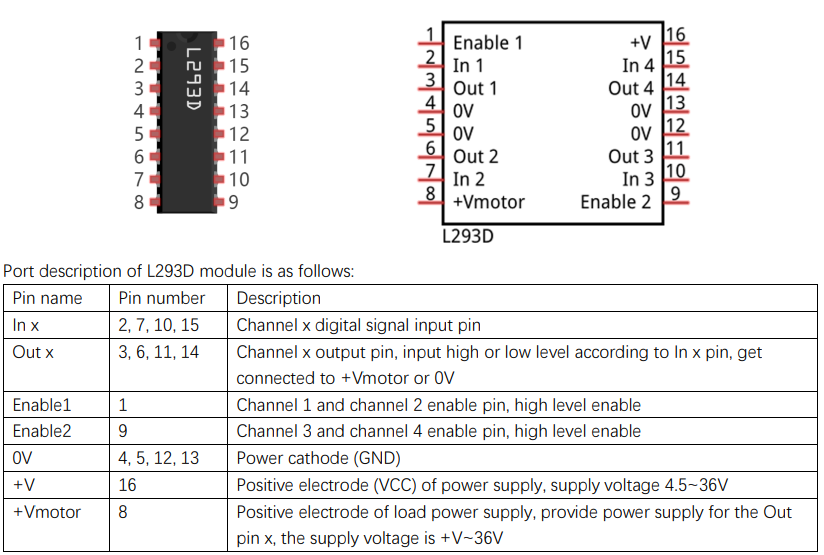
\includegraphics[width=8.5cm]{../images/L293D.png}
\caption{L293D Schaltplan}
\label{Elektrik:L293D}
\end{figure}

\subsection{Pulsweitenmodulation}

PWM (Pulsweitenmodulation) ermöglicht die präzise Steuerung der Drehgeschwindigkeit eines Motors. Dabei wird kein konstantes Signal an den Motor angelegt,
sondern das Signal periodisch zwischen den Zuständen "An" und "Aus" gewechselt. Die Drehgeschwindigkeit wird durch die Anpassung der Pulsweiten innerhalb der Perioden 
bestimmt \autocite{611797}. Aufgrund der hohen Frequenz wird ein konstante Drehbewegung erreicht. 

In der aktuellen Konfiguration werden jedoch nur zwei Geschwindigkeiten benötigt: Stillstand (0) und maximale Geschwindigkeit. 
Dies wird durch die entsprechende Taktfrequenz in der Software gesteuert und durch die Verbindung der 
spezifizierten Pins des Micro-Controllers mit Pin 2 des Treibers realisiert.

Die Ansteuerung des Motors über den Treiber wird mithilfe von Pin 1, Pin 2 und Pin 7 realisiert. 
Diese Pins werden mit Digitalsignalen vom Micro-Controller gesteuert.
\begin{itemize}
  \item Pin 1 ist für die generelle Aktivierung des Motors verantwortlich
  \item Pin 2 und Pin 7 steuern die jeweilige Drehrichtung des Motors
\end{itemize}

Die folgende Tabelle zeigt die Kombinationen der Zustände von Pin 1, Pin 2 und Pin 7 und die resultierende Motorbewegung:

\begin{table}[]
  \begin{tabular}{llll}
  \hline
  \textbf{Pin1} & \textbf{Pin2} & \textbf{Pin2} & \textbf{Motor Bewegung}         \\ \hline
  H             & H             & L             & Drehung im Uhrzeigersinn        \\
  H             & L             & H             & Drehung gegen den Uhrzeigersinn \\
  L             & X             & X             & Keine Drehung                   \\ \hline
  \end{tabular}
\end{table}

Hierbei steht "H" für den High-Zustand (1) und "L" für den Low-Zustand (0). Wenn Pin 1 auf Low (L) gesetzt wird, wird der Motor nicht gedreht.

\subsection{Achsenansteuerung}

Aufgurnd der höheren Gewichtslast und der Sicherstellung einer konstanten Geschiwndigkeit, werden die x und Y Achsen durch eine XM Motor betrieben.
Hierbei wird für jede Achse ein seperater Treiber benötigt.

Für die Z-Achse kann eine schwächere Variante des Motors verwendet werden, was wiedereum einen Treibe benötigen würde.

\subsection{Servo-Motor}

Als Alternative könnte ein Servo-Motor verwendet werden, der die Höhe der Z-Achse über einen Arm verändert. 
In diesem Fall könnte auf den Treiber verzichtet werden. Allerdings wäre die Systemkompatibilität mit der Mechanik aufgrund der Nicht-Fischertechnik-Teile nicht gegeben. 
Daher wurde trotz des zusätzlichen Treibers ein Fischertechnik DC Motor für die Z-Achse verwendet.

\subsection{Schaltplan}

Aufgrund der aufgeführten Anforderungen und Eigenschaft, ergibt sich folgender elektrischer Aufbau auf Basis des ESP32-WROVER-Boards.
\begin{center}
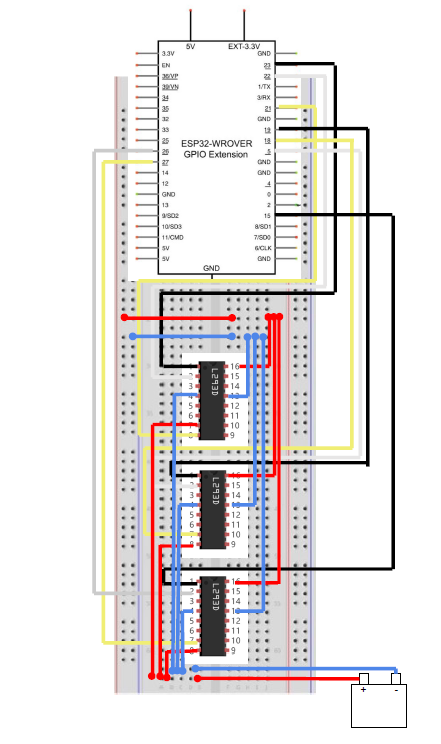
\includegraphics[width=8.5cm]{../images/schaltplan.png}
\caption{Schaltplan}
\label{Elektrik:Schaltplan}
\end{center}

\section{Softwaresteuerung}

\begin{itemize}
  \item WLAN & Bluetooth & Probleme
  \item Abstraktion Software Hardware
  \item Testbarkeit Software
  \item Wo hört Hardware Abstraktion auf und wo fängt Software an?
\end{itemize}

\subsection{Steuerung}

Für die Steuerung des Roboter standen verschiedene Methoden zur Verfügung. Die einzige Anforderung dabei
war es dass die Steuerung in der Lage ist die einzelnen Motoren und weitere Hardware Komponenten
zu kontrollieren. Hierzu haben wir uns folgende Möglichkeiten überlegt:

\begin{itemize}
  \item Steuerung über einen externen Computer
  \item Steuerung über eine mobile App
  \item Steuerung über einen Prozessor mit eingebautem Code
\end{itemize}

Die Steuerung über einen externen Computer wurde als erste Lösung betrachtet. Der Vorteil
ist hier, dass man auch eine vollfunktionsfähigens Betriebssystem mitsamt allen dafür existierenden
Paketen und Programmiersprachen zurückgreifen kann. Da aber das vollständige Betriebssystem auch
dazuführt, dass Services gestartet werden, die mit der eigentlichen Aufgabe des Roboters nichts zu
tun haben, wurde sich gegen diesen Ansatz entschieden. Zusätzlich erzwingt eine solche Steuerung
eine dauerhafte Verbindung zu dem Computer. Dies ist nicht erwünschens wert, da der Roboter autonom
handlungsfähig sein soll.

Als zweite Wahl kam die Steuerung über eine mobile App ins Spiel. Dies ermöglicht es, dass die
eigentlichen Bewegungen auf einem Gerät mit viel Prozessorstärke ausgeführt werden kann und dann nur
noch an den Roboter übermittelt werden muss. Somit ist auch der Zweck des Roboters
durch die Veränderung des Programmcodes auf dem Smartphone anpassbar. Die Schwachstelle hier ist,
dass weiterhin ein eingebetteter Prozess in Roboter vorhanden sein muss, der eine stabile
Kommunikation mit dem Mobilegerät besitzen muss. Während des Bau unseres Prototypen ist es den Autoren,
nicht gelungen eine stabile Kommunikation per Bluetooth mit einem iOS Gerät herzustellen.
Was die Nutzung des Roboters weiter einschränkt. Kommunikation per Wifi konnte hergestellt werden,
allerdings müssen sich sowohl das Mobiltelefon als auch der Roboter im 
selben Netzwerk befinden. Dies setzt eine Eingabemöglichkeit auf dem Roboter voraus oder dass
die Zugangsdaten vordefiniert sind. Beide Möglichkeiten sind in diesem Projekt nicht realisierbar,
da die Motorsteuerung schon alle Pins belegt und der während der Entwicklung und dem Einsatz in der
Hochschule in unterschiedlichen Netzwerken laufen können soll.

Letzlich fiel die Entscheidung darauf allen Code auf dem eingebetteten Chip zu spielen und dort
das gesamte Spiel zu implementieren. Dies bringt auch den Vorteil, dass der Roboter mit der Verbindung
zum Strom sofort spielbar ist. Außerdem werden so alle Fehlerfälle ausgeschlossen, die durch die
drahtlose Kommunikation zustande kommen könnten. Nachteilig ist hier, dass der Programmcode nur
vergleichsweise umständlich verändert werden kann. Da der Roboter nur für den aktuell singulären
Zweck des Tik-Tak-Toe spielen geschaffen wurde, wiegt dieser Nachteil allerdings nicht schwer.

\subsection{Tik-Tak-Toe Algorithmus}

Für den Tik-Tak-Toe Algorithmus wurde ein in C implementierter Algorithmus erstellt, der direkt auf
den ESP32-WROOM eingebettet wurde. Hierbei wurde großer Wert auf eine kompakte und einfache
Implementierung gelegt, da der gesamte Programmcode einschließlich des während der Laufzeit
gehaltenen Speichers in die 520KB Speicher des Chips passen mussten.

Um den Code einfach zu halten, wurde die Spielausführung auf einen der beiden CPU Kerne beschränkt.
Damit ist die Logik des Spiels einfach nachzuvollziehen, da sie von oben nach unten gelesen werden kann.
Um dieses Ziel zu erfüllen, wurden alle Bewegungen des Roboters als blockierende Calls im Programm
umgesetzt.

Kompakt wurde der Code gehalten, indem das Spielfeld in zwei einzelne 16Bit Integer integriert wurde.
Da das Spielfeld nur 9 Felder hat, werden nur 9Bit pro Spieler benötigt, um zu speichern, ob der Spieler
auf dem jeweiligen Feld aktiv ist. Damit sind 16Bit Integer die kleinst mögliche Speichereinheit, in der
diese Daten für einen Spieler gespeichert werden kann. Alle möglichen Gewinnstellungen werden entsprechend
auch von einem einzelnen 16Bit Integer repräsentiert. Um herauszufinden, ob ein Spieler gewonnen hat, kann
nun die Gewinnposition per bitweisem UND mit dem Spielfeld vergleichen und wenn das Ergebnis der Operation
der Gewinnposition entspricht, hat der Spieler diese erreicht.

Bei einem Spiel zwischen Mensch und Maschine nutzt der Roboter die enthaltenen Gewinnpositionen als
Entscheidungsgrundlage für den nächsten Zug. Dabei wird geprüft, welche der Gewinnpositionen noch erreichbar
sind. Danach wird ermittelt, wie viele Züge dazu noch zu ziehen sind. Die Gewinnposition mit den
wenigsten Zügen wird versucht zu erreichen. Falls mehrere Gewinnpositionen gleich gut gewichtet wurden
oder noch kein Zug gespielt wurde, wird zufällig eine Zielposition ausgewählt. Die Berechnung läuft
dabei nach jedem Zug, wodurch der Roboter auf dem Zug seines Gegners reagieren kann.

\subsection{Abstraktion Hardware & Software}

Um den Autoren die Möglichkeit zu geben, zu unterschiedlichen Zeitpunkten an dem Roboter arbeiten
zu können, wurde die Software und die Hardwareentwicklung per Abstraktionsstufe getrennt. Hierbei wurde
ein mindestmaß an Funktionalitäten definiert, die der Roboter bereitstellen können muss, um Tik-Tak-Toe
ausführen zu können. Diese Funktionalität wurde dann als Schnittstelle zwischen der Hardware und Software
genutzt. Damit wurde eine unabhängige Entwicklung der Softwarefunktionalität von der Hardware geschaffen.

Die Schnittstelle lässt sich in 4 Teile unterteilen.

\begin{verbatim}
void waitUntilGameStarts();
int getFieldSelectedByPlayer();
\end{verbatim}

Der oben aufgeführten erste Teil beinhaltet Funktionen, deren Aufgabe alle Nutzereingaben abdecken.
Ihre Aufgabe ist es so lange die weitere Ausführung des Programms zu blockieren,
bis ein Spiel gestartet werden kann oder bis der Nutzer ein Feld gewählt hat.

In diesen Funktionen wurden später auch die Möglichkeit eingebaut, alle Achsen des Roboters von 
Hand zu steuern, um ihn richtig ausrichten zu können. Dies ermöglicht es, dass hardware-nahe Funktionen
nicht im Spielalgorithmus verankert werden müssen und dennoch gut eingebaut werden konnten.

\begin{verbatim}
void moveRobotArmToOrigin();
void moveRobotArmToFieldOne();
void moveRobotArmToFieldTwo();
void moveRobotArmToFieldThree();
void moveRobotArmToFieldFour();
void moveRobotArmToFieldFive();
void moveRobotArmToFieldSix();
void moveRobotArmToFieldSeven();
void moveRobotArmToFieldEight();
void moveRobotArmToFieldNine();
\end{verbatim}

Im aufgeführten zweiten Teil, sind alle Funktionen beinhaltet, die Bewegungen des Roboter darstellen, um zu
einem bestimmten Spielfeld und wieder zurück zu kommen. Zu beachten ist hier, dass die Hardware den aktuellen
Ort des Stiftes kennen muss, um diesen nach dem entsprechenden Funktionsaufruf wieder zurück zum Ausgangspunkt
navigieren zu können.

Dies ist der dritte Teil:

\begin{verbatim}
void drawCross();
void drawCircle();
void drawStraightWinningLine();
void drawTopToBottomWinningLine();
void drawBottomToTopWinningLine();
\end{verbatim}

Der dritte Teil der Schnittstelle beschäftigt sich mit den Zeichenanweisungen des Roboters. Hierbei legt der
Tik-Tak-Toe Algorithmus fest, was gezeichnet werden soll. Die exakten Details der Bewegung und wann der Stift
auf das Blatt abgesetzt und gehoben werden muss, wurden auch hier als hardware-spezifisch deklariert.

\begin{verbatim}
void showCannotPlayMove();
\end{verbatim}

Zu letzt benötigt der Roboter eine Möglichkeit zu kommunizieren, dass ein Spielzug nicht gespielt werden kann,
weil dieser schon von einem anderen Spieler zuvor gespielt wurde. Dies stellt den vierten und letzten Teil der
Schnittstelle dar.

Die Aufteilung der Schnittstelle ermöglicht dabei nicht nur die getrennte Entwicklung von Hardware und Software,
sondern auch, dass die Software extern und automatisiert getestet werden konnte. Damit wurde die Funktionalität des Algorithmus
sichergestellt und erlaubte eine Test-basierte-Entwicklung auf einem leistungsstarken Computer ohne direkten
Hardwarezugriff zu benötigen.

\section{Fazit und Ausblick}
\begin{itemize}
  \item Offene Probleme
  \item Nutzung als Plotter
\end{itemize}

% Abschnitte mit \section, Unterabschnitte mit \subsection und
% Unterunterabschnitte mit \subsubsection
% -------------------------------------------------------
\section{Einleitung}
Die Einleitung liefert eine generelle Darstellung des Problems, der Ziele der Arbeit und deren Aufbau. Beschreibt den Hintergrund der Arbeit, das bearbeitete Problem und die Untersuchungsmethoden. Am Ende wird kurz der Aufbau der Arbeit erläutert.

Die Einleitung schreibt man erst, nachdem der Hauptteil der Arbeit fertig ist.

% -------------------------------------------------------
\section{Schreibstil}
\subsection{Zielgruppe}
Schreiben Sie die Arbeit so, dass ein fachkundiger Dritter in der Lage ist, den Text zu verstehen und die darin enthaltenen Schlüsse nachvollziehen zu können. Hierzu sollten alle nicht bekannten Fakten mit Literaturstellen belegt werden (\autoref{quellen}).

\subsection{Sprache}
Schreiben Sie in einer einfachen, gut verständlichen Sprache mit kurzen Sätzen. Schreiben sie durchgängig in der Gegenwartsform und im Aktiv (z.\,B. \enquote{\dots wird untersucht}, \enquote{\dots zeigt folgende Ergebnisse}). Nutzen Sie wenn möglich deutsche Begriffe, auf keinen Fall jedoch Mischformen wie \emph{downgeloaded} oder \emph{upgedatet}. Wenn es keinen guten deutschen Begriff gibt, dann verwenden Sie die englische Version, \zb Repository, Interrupt, etc.

\subsection{Gliederung}
Gliedern Sie die Arbeit nach logischen Kriterien. Die Gliederung der Arbeit erfolgt über \lstinline+\section{}+, \lstinline+\subsection{}+, \lstinline+\subsubsection{}+ und \lstinline+\paragraph{}+.

\subsection{Qualitätssicherung}
Zur Qualitätssicherung Ihrer Arbeit ist u.\,a. folgende Vorgehensweise hilfreich:
\begin{itemize}
\item Wenn es irgendwie möglich ist, sollten Sie die Arbeit auch Kommilitonen lesen lassen. Selbst Verwandte, Freunde und Bekannte, die nicht \emph{vom Fach} sind, finden vielleicht Fehler oder kommentieren Ihre Arbeit.
\item Um sicher zu stellen, dass Sie die hier beschriebenen Aspekte beachten, sollten Sie die Formalien z.\,B. nach jedem geschriebenen Kapitel überprüfen.
\item Lassen Sie sich von Ihrem betreuenden Professor alle Randbedingungen und Bewertungsschemata geben und fragen Sie, worauf sie achten sollen.
\end{itemize}



% -------------------------------------------------------
\section{Zitate und Quellenangaben}\label{quellen}
Alle von anderen Autoren gewonnenen Erkenntnisse müssen mit Quellen belegt werden. Falls Sie wörtlich zitieren werden, so muss der Text originalgetreu in Anführungszeichen wiedergegeben werden. Wird ein Teil des Textes ausgelassen, so werden Punkte in eckigen Klammern [\,\dots] an die Stelle der Auslassung gesetzt. Zusätze innerhalb des zitierten Textes bedürfen eckiger Klammern []. Gehen Sie sparsam mit wörtlichen Zitaten um. Längere wörtliche Zitate werden i.\,a. eingerückt. Hierzu dient die \textit{quotation}-Umgebung.

\begin{quotation}
Dies ist ein längeres Zitat, dass in einer Quotation-Umgebung gesetzt wurde. Es hat keine Anführungszeichen aber am Ende natürlich eine Quellenangabe \cite{Kornmeier2011}.
\end{quotation}

Die Zitierweise muss im gesamten Text einheitlich sein.

Wichtig ist, dass das Übernehmen von fremden Textstellen ohne entsprechende Kennzeichnung der Herkunft in einer wissenschaftlichen Arbeit nicht akzeptabel ist. Plagiate werden mit der Note 5.0 bewertet.

\subsection{Zitate im Text}
Wichtig ist das korrekte Zitieren von Quellen, wie es auch von \cite{Kornmeier2011} dargelegt wird. Interessant ist in diesem Zusammenhang auch der Artikel von \cite{Kramer2009}. Häufig werden die Zitate auch in Klammern gesetzt, wie bei \parencite{Kornmeier2011} und mit Seitenzahlen versehen \parencite[S. 22--24]{Kornmeier2011}.
Damit hier auch wissenschaftliche Arbeiten zitiert sind, sei hier auf eine Journal-Veröffentlichung \cite{Christidis2016} und einen Konferenzbeitrag \cite{Redmon2016} verwiesen.

In manchen Fällen (zur Illustration oder Visualisierung) könnte auch ein YouTube-Video\autocite{gronkh2019} als Quelle vorkommen.

Bei Webseiten wird auch die URL und das Abrufdatum mit angegeben \parencite{Gao2017}. Wenn die URL nicht korrekt umgebrochen wird, lohnt es sich, an den Parametern \textit{biburl*penalty} in der \texttt{preambel.tex} zu drehen. Kleinere Werte erhöhen die Wahrscheinlichkeit, dass getrennt wird.

Verwenden Sie das wörtliche Zitat nur dann, wenn es aus dem Kontext heraus sinnvoll ist, also z.\,B. um eine besondere Definition herauszustellen, oder eine sehr prägnante Aussage zu zitieren. Im Allgemeinen benötigen Sie kein wörtliches Zitat -- das macht Ihre Arbeit nur schwer zu lesen.

Insbesondere bei fremdsprachigen Quellen sollten Sie keine Original-Sätze zitieren, um sie dann mit eigenen Worten im Deutschen zu wiederholen (Ausnahme wie oben, wenn etwa die Wortwahl oder die Aussage besonders prägnant ist). Statt dessen sollten Sie den Text in ihren eigenen Worten in Deutsch formulieren, und dann die Quelle angeben.

Verwenden Sie die Namen des Autors/der Autoren nur dann, wenn

\begin{enumerate}
\item Sie es wichtig finden, zu sagen, dass diese Aussage von genau diesem Autor/diesen Autoren getroffen wurde (etwa bei einer Definition, oder bei einer Gegenüberstellung) oder
\item Sie deutlich machen wollen, dass die Aussage nicht von Ihnen stammt (was man aus dem Kontext sonst eventuell missverstehen könnte).
\end{enumerate}

Verwenden Sie Seitenzahlen bei der Angabe einer Quelle nur dann, wenn das für das Verständnis wichtig ist. Entnehmen Sie \enquote{Wissen} aus einem Paper an mehreren Stellen, dann reicht die Angabe des Papers. Ist es wichtig, die Stelle zu markieren (z.B. weil ein bestimmtes Argument referenziert wird), dann ergänzen Sie die Seite.

Insgesamt kann man sagen, dass Sie Sachverhalte mit eigenen Worten formulieren sollen, und jeweils kennzeichnen, wo der \enquote{Input} hergekommen ist. Eine explizite Nennung von Autor ist nur dann erforderlich, wenn es auch Sinn macht, diesen hervorzuheben.

Damit sollten Sie ein Plagiat vermeiden können, ohne extensiv zu zitieren. Umgekehrt schützt extensives Zitieren auch nicht vor einem Plagiat (z.\,B. wenn Sie einen englischen Text in Google Translation stecken, den übersetzten Text als Ihren eigenen ausgeben, und dann die Quelle ergänzen, ist das ein Plagiat).

\subsection{Zitierstile}
Verwenden Sie eine einheitliche und im gesamten Dokument konsequent durchgehaltene Zitierweise. Es gibt eine ganze Reihe von unterschiedlichen Standards für das Zitieren und den Aufbau eines Literaturverzeichnisses. Sie können entweder mit Fußnoten oder Kurzbelegen im Text arbeiten. Welches Verfahren Sie einsetzen ist Ihnen überlassen, nur müssen Sie es konsequent durchhalten.

In der Informatik ist das Zitieren mit Kurzbelegen im Text (Harvard-Zitierweise) weit verbreitet, wobei für das Literaturverzeichnis häufig die Regeln der \acs{ACM} oder \acs{IEEE} angewandt werden.\footnote{Einen Überblick über viele verschiedene Zitierweisen finden Sie in der \url{http://amath.colorado.edu/documentation/LaTeX/reference/faq/bibstyles.pdf}}

Am einfachsten ist es, wenn Sie das \lstinline+\autocite{}+-Kommando verwenden. Bei diesem Kommando können Sie in der Datei \texttt{perambel.tex} festlegen, wie die Zitate generell aussehen sollen, \zb ob sie in Fußnoten erfolgen sollen oder nicht. Wollen Sie von dem globalen Zitierstil abweichen, können Sie weiterhin spezielle Kommandos benutzen:

\begin{itemize}
	\item \lstinline+\autocite{Willberg1999}+: \autocite{Willberg1999}
	\item \lstinline+\cite{Willberg1999}+: \cite{Willberg1999}
	\item \lstinline+\parencite{Willberg1999}+: \parencite{Willberg1999}
	\item \lstinline+\footcite{Willberg1999}+: \footcite{Willberg1999}
	\item \lstinline+\citeauthor{Willberg1999}+: \citeauthor{Willberg1999}
	\item \lstinline+\citeauthor*{Willberg1999}+: \citeauthor*{Willberg1999}
	\item \lstinline+\citetitle{Willberg1999}+: \citetitle{Willberg1999}
	\item \lstinline+\fullcite{Willberg1999}+: \fullcite{Willberg1999}
\end{itemize}

\textit{Für die Veranstaltung WIA ist der Zitierstil mit IEEE festgelegt und Sie sollten die Einstellungen am Template nicht verändern. Am besten, Sie verwenden einfach}  \lstinline+\autocite{}+ \textit{und machen sich dann keine Gedanken mehr um den Stil.}

\subsection{Zitieren von Internetquellen}
Internetquellen sind normalerweise \textit{nicht} zitierfähig. Zum einen, weil sie nicht dauerhaft zur Verfügung stehen und damit für den Leser möglicherweise nicht beschaffbar sind und zum anderen, weil häufig der wissenschaftliche Anspruch fehlt.\footnote{Eine lesenswerte Abhandlung zu diesem Thema findet sich (im Internet) bei \autocite{Weber2006}.}

Wenn ausnahmsweise doch eine Internetquelle zitiert werden muss, z.\,B. weil für eine Arbeit dort Informationen zu einem beschriebenen Unternehmen abgerufen wurden, sind folgende Punkte zu beachten:

\begin{itemize}
\item Die Webseite ist auszudrucken und im Anhang der Arbeit beizufügens oder als PDF zusammen mit der Arbeit auf einem Datenträger einzureichen,
\item das Datum des Abrufs und die URL sind anzugeben,
\item verwenden Sie Internet-Seiten ausschließlich zu illustrativen Zwecken (z.\,B. um einen Sachverhalt noch etwas genauer zu erläutern), aber nicht zur Faktenvermittlung (z.\,B. um eine Ihrer Thesen zu belegen).
\end{itemize}

Wenn Sie aufgrund der Natur Ihrer Arbeit sehr viele Internetquellen benötigen, dann können Sie diese statt sie auszudrucken auch in elektronischer Form ablegen.

Wikipedia stellt einen immensen Wissensfundus dar und enthält zu vielen Themen hervorragende Artikel. Sie müssen sich aber darüber im Klaren sein, dass die Artikel in Wikipedia einem ständigen Wandel unterworfen sind und nicht als Quelle für wissenschaftliche Fakten genutzt werden sollten. Es gelten die allgemeinen Regeln für das Zitieren von Internetquellen. Sollten Sie doch Wikipedia nutzen müssen, verwenden Sie bitte ausschließlich den Perma-Link\footnote{Sie erhalten den Permalink über die Historie der Seite und einen Klick auf das Datum.} zu der Version der Seite, die Sie aufgerufen haben.

\subsection{Wo kommt die Quelle hin?}
Wo werden die Quellen zu einem Zitat bzw. die Belege zu einer Aussage platziert?

\begin{itemize}
\item Wenn die Quelle sich auf den ganzen Satz bezieht: Am Ende des Satzes \textit{vor} dem Punkt:\\ \textit{Ein Muggle ist ein Mensch ohne Zauberkräfte [1, S. 124]. Ein Dementor ist ein Untoter [2, S. 234].}
\item Wenn der Autor herausgestellt werden soll: Am Anfang des Satzes:\\ \textit{Rowling [2, S. 234] beschreibt den Muggle als Menschen ohne Zauberkräfte.}
\item Wenn der Autor herausgestellt werden soll aber der Absatz lang ist, am Ende des Absatzes:\\ \textit{Rowling beschreibt den Muggle als Menschen ohne Zauberkräfte... [2, S. 234].}
\item Wenn die Quelle sich auf ein \textit{kurzes} wörtliches Zitat bezieht, direkt nach dem Zitat, vor dem Punkt:\\ \textit{Hermine behauptet, dass \enquote{Harry Potter der weltgrößte Zauberer} [1, S. 20] sei.}
\item Wenn die Quelle sich auf einen Begriff oder Teil des Satzes bezieht, direkt \textit{nach dem Begriff}, auf den sich die Quelle bezieht:\\ \textit{Man unterscheidet bei Harry Potter Muggle [2, S. 124] und Zauberer [2, S. 133].}
\item Wenn es sich um ein langes wörtliches Zitat handelt, wird es eingerückt und ohne Anführungszeichen gesetzt, wobei die Quelle am Ende angegeben wird. Hierzu verwendet man die \texttt{quote}-Umgebung in \LaTeX.
\end{itemize}

% -------------------------------------------------------
\section{Typographie}
\subsection{Hervorhebungen}\label{Einleitung:Textauszeichnungen}
Achten Sie bitte auf die grundlegenden Regeln der Typographie\footnote{Ein Ratgeber in allen Detailfragen ist \cite{Forssman2002}.}, wenn Sie Ihren Text schreiben. Hierzu gehören \zb die Verwendung der richtigen "`Anführungszeichen"' und der Unterschied zwischen Binde- (-), Gedankenstrich (--) und langem Strich (---).

Wenn Sie Text hervorheben wollen, dann setzten Sie ihn \textit{kursiv} (Italic) und nicht \textbf{fett} (Bold). Fettdruck ist Überschriften vorbehalten; im Fließtext stört er den Lesefluss. Das \underline{Unterstreichen} von Fließtext ist im gesamten Dokument tabu und kann maximal bei Pseudo-Code vorkommen.

\subsection{Anführungszeichen}
Deutsche Anführungszeichen gehen so: "`dieser Text steht in \glq Anführungszeichen\grq; alles klar?"'. Englische Anführungszeichen werden anders benutzt: ``this is an `English' quotation.''

Am besten Sie verwenden das Paket \textit{csquotes}, dass über das Makro \lstinline+\enquote+ immer die richtigen \enquote{Anführungszeichen} bietet und auch die Spracheinstellungen berücksichtigt. Sie können mehrere Anführungszeichen ineinander schachteln: \enquote{Und der Almöhi sagte \enquote{Heidi, komm heim} und steckte sich die Pfeife an.}.

\subsection{Abkürzungen}
Abkürzungen müssen in einem Ab"-kürzungs"-verzeichnis aufgeführt und bei der ersten Verwendung auch ausgeschrieben werden, also z.\,B. \ac{AES} bei der ersten Verwendung, danach einfach nur \ac{AES}. Man kann allerdings die Langform explizit anfordern: \acl{ABK} oder die Kurzform \acs{ABK} oder auch noch einmal die Definition: \acf{ABK}.

Beachten Sie, dass bei Abkürzungen, die für zwei Wörter stehen, ein kleines Leerzeichen nach dem Punkt kommt: z.\,B. bzw. \zb, d.\,h. bzw. \dahe

\subsection{Querverweise}
Querverweise auf eine Kapitelnummer macht man im Text mit \lstinline+\ref+ (Kapitel~\ref{Einleitung:Textauszeichnungen}) und auf eine bestimmte Seite mit \lstinline+\pageref+ (Seite~\pageref{Einleitung:Textauszeichnungen}). Man kann auch den Befehl \lstinline+\autoref+ benutzen, der automatisch die Art des referenzierten Elements bestimmt (\zb \autoref{Einleitung:Textauszeichnungen}).

\subsection{Fußnoten}
Fußnoten werden einfach mit in den Text geschrieben und zwar genau an die Stelle\footnote{an der die Fußnote auftauchen soll.}

\subsection{Fremdsprachige Begriffe}
Wenn Sie Ihre Arbeit auf Deutsch verfassen, gehen Sie sparsam mit englischen Ausdrücken um. Natürlich brauchen Sie etablierte englische Fachbegriffe, wie z.\,B. \textit{Interrupt}, nicht zu übersetzen. Sie sollten aber immer dann, wenn es einen gleichwertigen deutschen Begriff gibt, diesem den Vorrang geben. Den englischen Begriff (\textit{term}) können Sie dann in Klammern oder in einer Fußnote\footnote{Englisch: \textit{footnote}.} erwähnen. Absolut unakzeptabel sind deutsch gebeugte englische Wörter oder Kompositionen aus deutschen und englischen Wörtern wie z.\,B. downgeloadet, upgedated, Keydruck oder Beautyzentrum.

\subsection{Tabellen}
Tabellen werden normalerweise ohne vertikale Striche gesetzt, sondern die Spalten werden durch einen entsprechenden Abstand voneinander getrennt.\footnote{Siehe \cite[S. 89]{Willberg1999}.} Zum Einsatz kommen ausschließlich horizontale Linien (siehe \autoref{google:numbers}). Beachgen Sie, dass bei Tabellen -- anders als bei Abbildungen -- die Beschriftung über der Tabelle steht.

% Tabelle
\begin{table}[!ht]
\centering
\rmfamily
\caption{Zeitbedarf für ausgewählte Aktionen, nach~\cite{Dean2012}}
\renewcommand{\arraystretch}{1.1}
\sffamily
\begin{footnotesize}
\begin{tabular}{l r}
\toprule
\textbf{Vorgang} & \textbf{Zeitbedarf} \\
\midrule
L1 cache reference                  & 0,5 ns\\
Branch mispredict                   & 5 ns\\
L2 cache reference                  & 7 ns\\
Mutex lock/unlock                   & 100 ns\\
Main memory reference               & 100 ns\\
Compress 1K bytes with Zippy        & 10.000 ns\\
Send 2K bytes over 1 Gbps network   & 20.000 ns\\
Read 1 MB sequentially from memory  & 250.000 ns\\
Round trip within same datacenter   & 500.000 ns\\
Disk seek                           & 10.000.000 ns\\
Read 1 MB sequentially from network & 10.000.000 ns\\
Read 1 MB sequentially from disk    & 30.000.000 ns\\
Send packet CA-Netherlands-CA       & 150.000.000 ns\\
\bottomrule
\end{tabular}
\end{footnotesize}
\label{google:numbers}
\end{table}

\subsection{Aufzählungen}
Aufzählungen werden mit der \texttt{itemize}-Umgebung erzeugt und können auch einfach ineinander geschachtelt werden.

\begin{itemize}
  \item Ein wichtiger Punkt
  \item Noch ein wichtiger Punkt
  \item Ein Punkt mit Unterpunkten
    \begin{itemize}
      \item Unterpunkt 1
      \item Unterpunkt 2
    \end{itemize}
  \item Ein abschließender Punkt ohne Unterpunkte
\end{itemize}

Aufzählungen mit laufenden Nummern sind mit der \texttt{enumerate}-Umgebung möglich.

\begin{enumerate}
  \item Ein wichtiger Punkt
  \item Noch ein wichtiger Punkt
  \item Ein Punkt mit Unterpunkten
    \begin{enumerate}
      \item Unterpunkt 1
      \item Unterpunkt 2
    \end{enumerate}
  \item Ein abschließender Punkt ohne Unterpunkte
\end{enumerate}

\subsection{Abbildungen}
Abbildungen sind oft sehr hilfreich, um Zusammenhänge zu verdeutlichen. Soweit möglich, sollten die Abbildungen als Vektorgrafiken eingebunden werden. Die in der Abbildung enthaltenen Schriftarten sollten nach Möglichkeit die gleichen sein, wie im restlichen Dokument. Alle Beschriftungen innerhalb der Grafik sollten gut lesbar sein.
Graphen können farbig sein, wenn es der Lesbarkeit dient. Es sollte jedoch darauf geachtet werden, dass auch eine schwarz\-weiß-Kopie noch alle nötigen Informationen enthält (d.h. Liniendiagramme mit verschiedenen Linienarten z.\,B. Strichpunkt).
Falls eine Abbildung nur in Form einer Bitmap realisiert werden kann (z.\,B. Screenshot), sollte die Auflösung mindestens 600 dpi betragen und die Qualität nicht durch Komprimierung (z.\,B. jpg) verschlechtert werden. Unkomprimierte oder verlustfrei komprimierte Bildformate wie \emph{png} oder \emph{bmp} sind zu bevorzugen. Nur für echte Fotos ist \emph{jpg} geeignet.

% Grafik in einer Spalte
\begin{figure}[!ht]
\centering
\includegraphics[width=8.5cm]{bsp1}
\caption{Beispielgrafik~\cite{Dean2012}}
\label{fig_sim}
\end{figure}

Jede Abbildung (vgl. \autoref{fig_sim} auf Seite~\pageref{fig_sim}) und Tabelle (z.\,B. \autoref{google:numbers} auf Seite~\pageref{google:numbers}) sollte im Fließtext referenziert und beschrieben/erläutert werden. Die Beschriftung unter den Abbildungen sollte die Abbildung vollständig und verständlich beschreiben, auch ohne dass man den restlichen Text gelesen hat. Gleiches gilt für die Beschriftungen von Tabellen, die über die Tabellen gesetzt werden.

\subsection{Formelsatz}
Eine Formel gefällig? Mitten im Text $a_2 = \sqrt{x^3}$ oder als eigener Absatz (siehe Formel~\ref{Formel}):

\begin{equation}
\begin{bmatrix}
   1 &  4 &  2 \\
   4 &  0 & -3
\end{bmatrix}
        \cdot
\begin{bmatrix}
   1 &  1 &  0 \\
  -2 &  3 &  5 \\
   0 &  1 &  4
\end{bmatrix}
       {=}
\begin{bmatrix}
  -7 &  15 &  28 \\
   4 &   1 & -12
\end{bmatrix}
\label{Formel}
\end{equation}

% --------------------------------------------------------------------
\section*{Abkürzungen}
\addcontentsline{toc}{section}{Abkürzungen}

% Die längste Abkürzung wird in die eckigen Klammern
% bei \begin{acronym} geschrieben, um einen hässlichen
% Umbruch zu verhindern
% Sie müssen die Abkürzungen selbst alphabetisch sortieren!
\begin{acronym}[IEEE]
\acro{A2A}{Application-to-Application}
\acro{ABK}{Abkürzung}
\acro{ACL}{Acess Control List}
\acro{ACM}{Association of Computing Machinery}
\acro{AES}{Advanced Encryption Standard}
\acro{IEEE}{Institute of Electrical and Electronics Engineers}
\acro{ISO}{International Organization for Standardization}
\acro{PDF}{Portable Document Format}
\end{acronym}

% Literaturverzeichnis
\addcontentsline{toc}{section}{Literatur}
\printbibliography

\end{document}
